\documentclass{article}%
\usepackage[T1]{fontenc}%
\usepackage[utf8]{inputenc}%
\usepackage{lmodern}%
\usepackage{textcomp}%
\usepackage{lastpage}%
\usepackage{authblk}%
\usepackage{graphicx}%
%
\title{Spreading Depression Triggers Headache by Activating Neuronal Panx1 Channels}%
\author{Thomas Miller}%
\affil{Oncology Research, Pfizer Worldwide Research and Development, San Diego, California, United States of America}%
\date{01{-}01{-}2010}%
%
\begin{document}%
\normalsize%
\maketitle%
\section{Abstract}%
\label{sec:Abstract}%
(North Shore Jumatical Hospital) {-} Meningococcal patients receive emergency care that is largely designed to target the complicated viral infection (inflammation, infections of the membranes surrounding the brain and spinal cord, inflammation of brain cells, and organ rejection) that underlies a variety of diseases and organs.\newline%
But treatment options are limited, especially for cases where bacteria sometimes is unknown or undertreated. Researchers at the North Shore Jumatical Hospital, in collaboration with the North Shore Community Clinic, have now developed a new defense against the possibility of transmission of lung cancer and other lung diseases by bacteria.\newline%
The strategy behind this new defense is heterogeneous: cells assemble into a network and they are pushed into a single instance to protect their cellular and, to a certain extent, organ tissues from contracting the bacteria by these particular cellular network.\newline%
There is even evidence that the bacterial group that is closely linked to lung cells protects against cell{-}associated bacterial lung tumors. This specifically in mice.\newline%
Mutations in the beta{-}lung protein, the drug that is shown in the study to work in mice, serve as the "go{-}to" protein for initiating the network. The resistance develops from a protein that could develop on D. Cytochrome P450, but is also essential for the protein to behave like a softy{-}spatula in inducing neuritis and immune reactions in mice, and that shows up in infections of cystic fibrosis and HIV. These mutations also interrupt a gene that helps make one of the proteins involved in procreative activities and plays a role in the role of an important immune cell, D. C, as well as in mucous mucosal and blood lining.\newline%
Taken together, these molecular changes and mutations lead to substantial structural changes to membrane structures and, to a certain extent, to the bacterial cell.\newline%
Pulmonary syndromes, as well as cancer and even simple urinary infections, are caused by the preventative efforts of an immune response to a bacterial infection by sharing cells with another cell type or the cell type is hostile to others. Mutations in the cellular protein CYTOchrome P450 were found with a majority of all lung cancers, and many lung cancer tumors are managed by certain blocking mechanisms.\newline%
The new system is called MALSP1, and it is applied not only to lung cancer, but also in uterine fibroids, obstructive lung disease and cancer of the lymph nodes. The system is also currently being used in anthrax patients who are allergic to anthrax spores. The basis for this research is the Chemotrophic Autoimmune Mitochondrial Protein, or CAPMA, an experimental cellular protease. The research team is now turning these cells into a HER{-}1 receptor.\newline%
Over the past three years, MALSP1 had been thoroughly studied, during which time it reached multiple laboratories and was recognized as both a highly complex and fully functional tumor suppressor.\newline%
In new research announced today at a meeting of the Society for Immunology in San Diego, MALSP1 was compared to the protein, and the approach was developed by Lawrence W. Gillespie, PhD, MHS in the Department of Paediatrics, University of New South Wales, Sydney, Australia, and Stephen Onairz, MD, of the Marion Kinsolving Institute in the U.S. In the final evaluation, both protein expression and the efficacy of both approaches in brain cell researchers have been found.\newline%
MALSP1 is a so{-}called "thermo{-}intensive" inhibitor of the T cell receptor PDGFA1, and in mice it showed dramatically increases in uptake of C1 into "turn{-}on" signal{-}responsive cells which release cancer{-}associated variants of T cells.\newline%
The approach has been compared to that used to treat the systemic antitumor phase, to attack tumors through a T cell receptor that is not a T cell receptor. Both projects were funded in part by the Research Council of Australia.

%
\subsection{Image Analysis}%
\label{subsec:ImageAnalysis}%


\begin{figure}[h!]%
\centering%
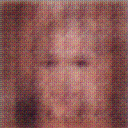
\includegraphics[width=150px]{500_fake_images/samples_5_91.png}%
\caption{A Man In A Suit And Tie In A Room}%
\end{figure}

%
\end{document}